\chapter{Technologien und Werkzeuge}
\label{cha:technologie_werkzeuge}
Die verwendeten Technologien und Werkzeuge sind für diese Arbeit wesentlich, um die Implementierung nachvollziehen zu können. Die Entwicklungsplattform .NET spielt dabei für das entwickelte Framework eine entscheidende Rolle, wie bereits in Unterabschnitt \ref{subsec:patterns} bei den beschriebenen Patterns erwähnt. In diesem Kapitel werden daher einige zentrale Konzepte vorgestellt. Der Schwerpunkt liegt insbesondere auf der Behandlung der verwendeten UI-Frameworks der .NET-Plattform.

\section{Visual Studio}
\label{sec:visual_studio}
Für C\# {Unterabschnitt \ref{subsec:csharp}} gibt es mehere Entwicklungsumgebung wie z.B. Ride und VisualStudio. Da der in dieser Arbeit erstellte Arbeit in eimen Produktiv Umfeld eingesetzt werden soll, in wlechen VisualStudio verwedet wird, wurde auch in dieser Arbeit Visual Studio für die Enwiclung eingesetzt. VisualStd

\section{.NET}
\label{sec:dotnet}
Für die Umsetzung der Implementierung in Kapitel \ref{cha:implementierung} wird die von Microsoft bereitgestellte Laufzeitumgebung und Entwicklungsplattform .NET \cite{dotnet} in der Version 8 \footnote{Microsoft veröffentlicht alle zwei Jahre eine Long-Term-Support-Version (LTS) von .NET. Version 8 wurde im November 2024 bereitgestellt und bietet langfristigen Support. Darüber hinaus erscheint jährlich im November eine neue .NET-Version.} verwendet. Diese Version enthält bereits die beiden UI-Frameworks WPF (siehe Unterabschnitt \ref{subsec:WPF}) und Windows Forms (siehe Unterabschnitt \ref{subsec:Winforms}), die ausschließlich unter Windows-Betriebssystemen eingesetzt werden können. Die für diese Arbeit relevanten Konzepte und Funktionen von .NET werden in diesem Kapitel näher erläutert.

\subsection{C\#}
\label{subsec:csharp}
Für die .NET-Plattform stehen mehrere Programmiersprachen zur Verfügung, darunter C\#, F\# und VB.NET. Für die Entwicklung des Frameworks wird C\# verwendet. Diese Sprache gilt laut Microsoft \cite{microsoft-tour-of-csharp} als die beliebteste Sprache innerhalb des .NET-Ökosystems und basiert auf dem objektorientierten Paradigma. Darüber hinaus integriert C\# Konzepte aus weiteren Programmierparadigmen, wie der funktionalen Programmierung. Ein Beispiel für die funktionale Programmierung ist Language Integrated Query (LINQ), das typisierte Abfragen in einer SQL-ähnlichen Syntax direkt im Code ermöglicht.

\subsubsection{Übersetzung und Ausführung}
C\# wird, wie auch andere Sprachen desselben Ökosystems, zunächst in IL (Intermediate Language) übersetzt. Dieser IL-Code wird anschließend durch die Common Language Runtime (CLR) \cite{microsoft-clr-overview} in nativen Maschinencode umgewandelt. Standardmäßig erfolgt diese Übersetzung in .NET über den Just-in-Time-Compiler (JIT). Es existieren jedoch auch Varianten, bei denen Anwendungen bereits teilweise oder vollständig vor der Ausführung in nativen Code kompiliert werden (Ahead-of-Time-Kompilierung \cite{microsoft-native-aot}).

Für die Ausführung von .NET-Programmen wird somit die CLR benötigt, die Bestandteil der .NET Runtime Environment bzw. des .NET SDK ist. Die Assemblies (siehe Unterabschnitt \ref{subsec:assemblies}) werden üblicherweise als \texttt{.dll}- oder \texttt{.exe}-Dateien abgelegt, unterscheiden sich inhaltlich jedoch von C++ Programmen, die nativ kompiliert werden.

\subsection{Nullable Reference Types}
Der bekannte Informatiker Tony Hoare bezeichnete die Einführung von \texttt{null} als seinen größten Fehler, da die dadurch verursachten Probleme enorm seien \cite{hoare_null_video}. Dieses Problem lässt sich bis zu einem gewissen Grad durch die sogenannten Nullable Reference Types \cite{microsoft-nullable-references} lösen. Der Compiler prüft hierbei, ob eine Variable den Wert \texttt{null} annehmen kann und falls dies der Fall ist, muss der Code explizit eine entsprechende Überprüfung vorsehen. Aufgrund der damit verbundenen Reduzierung von NullReferenceException-Fehlern wird dieses Konzept auch in dieser Arbeit verwendet. Entscheidend ist jedoch, dass die durch den Compiler entstehenden Warnings auf Errors umgestellt werden, um die Abdeckung aller entstandenen Nullszenarien zu garantieren.

\subsection{Assemblies}
\label{subsec:assemblies}
Die Erzeugnisse des Kompilierungsprozesses werden in .NET als Assemblies \cite{msdn_assembly_manifest} bezeichnet. Für Assemblies existieren zwei Dateitypen: \texttt{.dll} und \texttt{.exe}. Assemblies des Typs \texttt{.exe} sind ausführbare Dateien, während Assemblies des Typs \texttt{.dll} Klassenbibliotheken bzw. andere Programmteile darstellen, die wiederverwendet werden können.

\subsubsection{Erzeugung von Assemblies}
Abbildung \ref{fig:assemblies_dotnet} zeigt, wie eine Assembly aus mehreren Quelldateien erzeugt wird. Dabei wird das MSBuild-File verwendet, um dem Compiler die erforderlichen Schritte mitzuteilen. Der Compiler erzeugt anschließend aus den Ressourcen und den C\#-Dateien (siehe Unterabschnitt \ref{subsec:csharp}) eine Assembly. Dabei werden die Ressourcen, Metadaten und der IL-Code in die resultierende Datei eingebettet.

\subsubsection{Aufbau einer Assembly}
Eine Assembly besteht, wie in Abbildung \ref{fig:assemblies_dotnet} dargestellt, aus mehreren Modulen. Diese sogenannten Module enthalten IL-Code und Metadaten, wobei das Hauptmodul zusätzlich ein Manifest beinhaltet.  
Der IL-Code (Intermediate Language) stellt eine Zwischensprache zwischen Maschinencode und der Programmiersprache dar und enthält die Anweisungen, die letztlich ausgeführt werden.  
Die Metadaten enthalten Informationen über Methodensignaturen, Typen und weitere Strukturdaten. Diese Metainformationen bilden zusammen mit Reflection (siehe Unterabschnitt \ref{subsec:reflection}) einen wichtigen Bestandteil der Laufzeitumgebung. Weiters enthält das erwähnte Manifest folgende Informationen:

\begin{itemize}
    \item Assembly Name
    \item Assembly Version: Wesentlich, da Assemblies die kleinstmögliche Einheit der Versionierung darstellen. Dies ermöglicht beispielsweise die gleichzeitige Verwendung verschiedener Versionen einer Klassenbibliothek in einem Projekt, ohne dass Assemblies überschrieben werden.
    \item File Table: Listet die eingebetteten Ressourcen auf.
    \item References List: Listet die Abhängigkeiten zu anderen Assemblies auf.
    \item Modules: Gibt an, welche Module in einer Assembly enthalten sind. Im Standardfall, wie in Abbildung \ref{fig:assemblies_dotnet} dargestellt, existiert nur ein Modul.
\end{itemize}

Da Assemblies im PE-Format (Portable Executable) \cite{MicrosoftLearn_PEFormat} gespeichert werden, enthalten sie zusätzlich alle für dieses Format erforderlichen Informationen.

\begin{figure}[H]
    \centering
    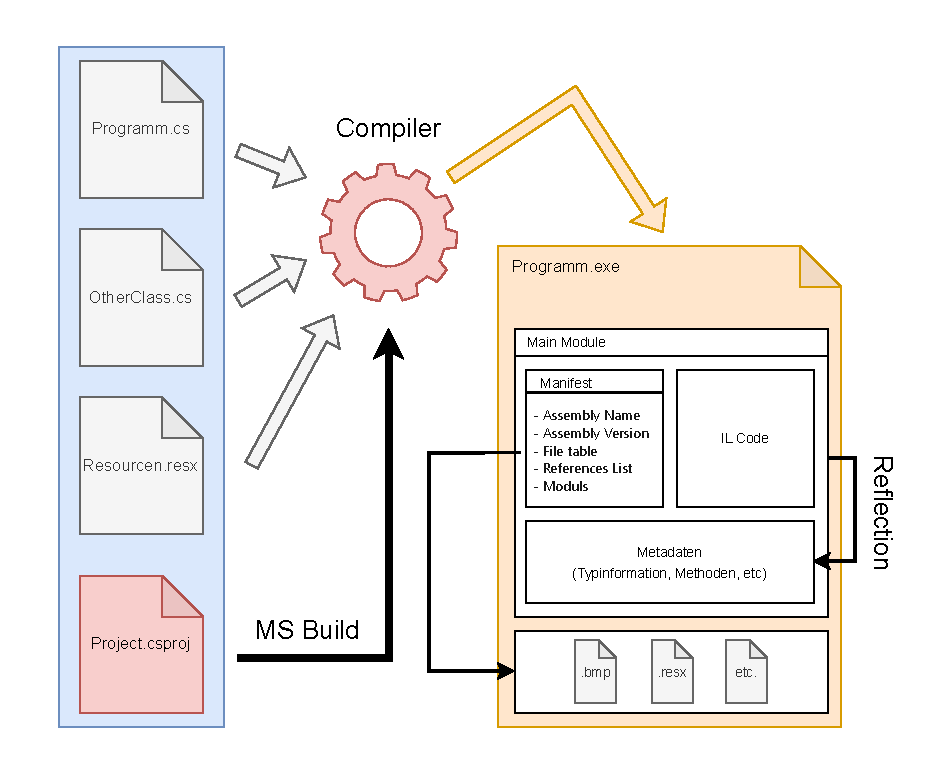
\includegraphics[width=0.9\textwidth]{2_Assemblies_Dotnet}
    \caption{Assemblies Aufbau und Generierung}
    \label{fig:assemblies_dotnet}
\end{figure}

\subsection{Reflection}
\label{subsec:reflection}
In Abbildung \ref{fig:assemblies_dotnet} zeigt ein Pfeil vom IL-Code zu den Metadaten. Dies verdeutlicht, dass in C\# (siehe Unterabschnitt \ref{subsec:csharp}) ein Mechanismus namens \textit{Reflection} \cite{MicrosoftLearn_Reflection} existiert, der es ermöglicht, Metainformationen über Typen, Methoden oder Attribute zur Laufzeit abzufragen und zu manipulieren. 

Reflection basiert auf speziellen IL-Instruktionen, die über die .NET-API auch in C\# zugänglich sind. Dadurch kann ein Programm beispielsweise alle Eigenschaften eines bestimmten Typs ermitteln und deren Werte dynamisch auslesen oder ändern. 

Reflection ist ein sehr mächtiges Werkzeug, bringt jedoch Leistungseinbußen mit sich. Der Zugriff auf Werte oder Typinformationen über Reflection ist deutlich langsamer als ein zur Compilezeit generierter Zugriff. Das liegt daran, dass die zugrunde liegenden Type- und MemberInfo-Objekte beim ersten Zugriff aus den Assembly-Metadaten erzeugt und anschließend zwischengespeichert werden müssen. Jeder weitere Zugriff erfolgt indirekt über mehrere Objekte, wodurch zusätzliche Zwischenschritte, ähnlich wie bei einer virtuellen Methodentabelle, notwendig werden. Die Auswirkungen von Reflection auf die Laufzeit werden in einem Artikel auf MSDN näher beschrieben \cite{Pobar2005_PerformancePitfalls}.


\subsection{Asynchrone Programmierung}
\label{subsec:async}

\section{UI Frameworks}
\label{sec:ui_frameworks}

\subsection{WPF}
\label{subsec:WPF}

\subsection{Windows Forms}
\label{subsec:Winforms}


